\newcommand*\circled[2][black]{\tikz[baseline=(char.base)]{
    \node[scale=0.85pt,shape=circle, thin,draw=#1!60, fill=#1!5,inner sep=0.1pt] (char) {#2};}}

\tikzset{
    linedot diameter/.store in=\linedot@diameter,
    linedot diameter=2pt,
    linedot spacing/.store in=\linedot@spacing,
    linedot spacing=16pt,
    linedots/.style={
        line width=\linedot@diameter,
        line cap=round,
        dash pattern=on 0pt off \linedot@spacing,
    }
}


\section{Neural Mass Models}\label{sec:neural-mass-models}

As already covered in the introduction,
neural mass models describe neuron populations and their interaction.
Their level of abstraction matches the signal recorded by EEG electrodes (compare Sec.~\ref{sec:eeg}),
as they generate summed PSPs of pyramidal cell populations.
Since we are looking to implement the Jansen-Rit Model and its extension by David \& Friston
for \ref{goal:jr_model} and \ref{goal:df_model}),
we must first explore their theoretical background.

\subsection{The Basic Jansen-Rit Model}\label{subsec:the-jansen-rit-model}

The Jansen-Rit Model~\cite{jansen_neurophysiologically-based_1993, jansen_electroencephalogram_1995}
represents a cortical column in the brain, which is made up of three main components,
each modeling a population of neurons with distinct characteristics.
This section introduces the model presented in~\cite{jansen_neurophysiologically-based_1993}
and~\cite{jansen_electroencephalogram_1995}.

The basic schema of the model is visualized in Fig.~\ref{fig:Jansen Rit Flowchart}, showing the connections
\begin{wrapfigure}{r}{0.5\textwidth}
    \begin{tikzpicture}[
		roundein/.style={circle, draw=green!60, fill=green!5, very thick, minimum size=11mm},
		roundiin/.style={circle, draw=red!60, fill=red!5, very thick, minimum size=11mm},
		rectp/.style={rectangle, rounded corners=2mm, draw=green!60, fill=green!5, very thick},
		trinode/.style={isosceles triangle, isosceles triangle apex angle=60, very thick, draw=cyan!60, shape border rotate=270, fill=cyan!5,},
		]
        
        \pgfdeclarelayer{bg}
        \pgfsetlayers{bg,main}
        
		%Nodes
		
		\node[trinode]    (PC)        {PC};
		\node[roundein]   (EIN)  [above left= 0.5cm and 2.25cm of PC.center] {EIN};
		\node[roundiin]   (IIN) [above right= 0.5cm and 2.25cm of PC.center] {IIN};
		\node[rectp]   (p) [above left=3cm and 1cm of PC.north] {Ext.};
		\node[below= 0.5cm of PC] (pc_out){};
		\node[above= 0.2cm of EIN.north] (ein_out){};
		\node[above= 0.2cm of IIN.north] (iin_out){};
		%Lines
		\draw[-, red] (IIN.north) -- (iin_out.center){};
		\draw[-, green] (EIN.north) -- (ein_out.center){};
		
		\draw[-{Stealth[scale=1.5]}, red] (iin_out.center) -| (PC.30) node[near end, right, black](output){$\circled[red]{$-$}$};
		\draw[-{Stealth[scale=1.5]}, green] (ein_out.center) -| (PC.155) node[near end, left, black](output){$\circled[green]{$+$}$};
		\draw[-{Stealth[scale=1.5]}, green] (p.east) -| (PC.140) node[pos=0.888, right, black](output){$\circled[green]{$+$}$};
		
		
		\draw[-, green] (PC.south) -- (pc_out.center){};% node[near start, right](output){$\circled{$+$}$};
		
		\draw[-{Stealth[scale=1.5]}, green] (pc_out.center) -| (EIN.south){} node[pos=0.85, right, black](output){$\circled[green]{$+$}$};
		\draw[-{Stealth[scale=1.5]}, green] (pc_out.center) -| (IIN.south){} node[pos=0.85, left, black](output){$\circled[green]{$+$}$};
        
        \begin{pgfonlayer}{bg}
        
        
        \filldraw [fill=darkgray!5,draw=darkgray]
            ($ (EIN.west) + (-0.2,1.7) $)
            rectangle ($ (IIN.east) + (0.2,-3) $);
        \node [above left=1.35cm and 0.2 of EIN.west, anchor=west, text=darkgray]{Cortical Column};
        \end{pgfonlayer}
		
	\end{tikzpicture}
    \caption{\textbf{Basic Schema of the Jansen-Rit Model:} Three populations of neurons}
    \label{fig:Jansen Rit Flowchart}
\end{wrapfigure}
between the main components.
There is a population of Pyramidal Cells which receives input from two populations of inter-neurons,
one of which is excitatory while the other is inhibitory.
Each of the inter-neuron-populations receives the output of the PC population.
Additionally, there is external excitatory input to the PC population from other regions of the brain.

The Block Diagram (Fig.~\ref{fig:Jansen Rit Simple}) shows the individual modules of the model.
A population consists of two types of blocks:
The \textit{PSP-Block} models the behavior of the synapses and neuronal somata.
It can be either excitatory or inhibitory and converts the incoming average pre-synaptic pulse density to
an average post-synaptic membrane potential by convolving it \iltodo{separate sentences} with an
impulse response function ($h_e(t)$ and $h_i(t)$, for excitation and inhibition respectively).
The second block (sometimes called \textit{Potential-To-Rate-Block} after it's functionality)
calculates the populations response to this stimulation, transforming the incoming
average membrane potential back into an average pulse density of action potentials.
It may be roughly viewed as a functional counterpart to the axon hillock by establishing a firing threshold
and is usually implemented by a Sigmoid Function ($Sigm$).
External input from other regions of the brain is represented by $p(t)$.
The Connectivity Constants $C_1$, $C_2$, $C_3$ and $C_4$ proportionally represent the
average number of synapses between the populations.
The signal most closely related to the EEG (and therefore the output variable)
is the summed average membrane potential of the PC population ($y_1(t)-y_2(t)$ in Fig.~\ref{fig:Jansen Rit Simple}).
In its basic configuration, the model is designed to produce sinusoidal $\alpha$-activity.
The following subsections will introduce the main components of the model in detail.
%\todo{explain neurophysiology why $EEG \approx y_1-y_2$, or reference back to explanation in EEG section}\\[1em]

\begin{figure}[H]
    \centering
    \begin{tikzpicture}[
        pc/.style={draw=black!80},
        ein/.style={draw=black!80},
        iin/.style={draw=black!80},
        pcLabel/.style={font=\small,text=black},
        einLabel/.style={font=\small,text=black},
        iinLabel/.style={font=\small,text=black},
        rectNode/.style={draw=black!80, thick},
        roundNode/.style={circle, draw=black!80, thick},
        ]
	    
 % Nodes
\node[rectNode, pc] (SigmPC) [label={[pcLabel]:PC}] {$Sigm$};
\node[rectNode, pc] (PSPPC) [right=1.8cm of SigmPC.east]{$h_e(t)$};
\node[rectNode, ein] (SigmEIN) [above=2cm of SigmPC.center, label={[einLabel]:EIN}]{$Sigm$};
\node[rectNode, iin] (SigmIIN) [below=2cm of SigmPC.center, label={[iinLabel]:IIN}]{$Sigm$};
\node[rectNode, ein] (PSPEIN) [above left= 0.5cm and 2cm of SigmPC.west]{$h_e(t)$};
\node[rectNode, iin] (PSPIIN) [below left= 0.5cm and 2cm of SigmPC.west]{$h_i(t)$};
\node[rectNode, rounded corners=3mm, ein] (ext) [left=2cm of PSPEIN.west, label={[einLabel]:Ext.}]{$p(t)$};
\node (inpIPSP) [left=0.8cm of PSPIIN.west]{};
\node (outPPSP) [right=1.2cm of PSPPC.east]{};
\node[roundNode, ein] (c1) [right=2cm of SigmEIN.east]{$C_1$};
\node[roundNode, ein] (c2) [left=2cm of SigmEIN.west]{$C_2$};
\node[roundNode, iin] (c3) [right=2cm of SigmIIN.east]{$C_3$};
\node[roundNode, iin] (c4) [left=2cm of SigmIIN.west]{$C_4$};

% add PC
\node[roundNode, pc] (addPC) [left=0.8cm of SigmPC.west]{};
\draw[-, black!80, thick, pc] (addPC.north west) -- (addPC.south east);
\draw[-, black!80, thick, pc] (addPC.north east) -- (addPC.south west);
% add Excitatory
\node[roundNode, ein] (addExc) [left=0.8cm of PSPEIN.west]{};
\draw[-, black!80, thick, ein] (addExc.north west) -- (addExc.south east);
\draw[-, black!80, thick, ein] (addExc.north east) -- (addExc.south west);

% add PC -> Sigm PC -> PSP PC
\draw[-{Stealth[scale=1.5]}, pc] (addPC.east) -- (SigmPC.west)node[coordinate, pos=0.3](measurepoint){};
\draw[-{Stealth[scale=1.5]}, pc] (SigmPC.east) -- (PSPPC.west);

% PSP PC -> y0
\draw[-{Stealth[scale=1.5]}, pc] (PSPPC.east) -- (outPPSP.center) node[pos=0.5, above, pcLabel]{\small$y_0(t)$};

% y0 -> C1 -> Sigm EIN
\draw[-{Stealth[scale=1.5]}, ein, fill=none] (outPPSP.center) |- (c1.east);
\draw[-{Stealth[scale=1.5]}, ein] (c1.west) -- (SigmEIN.east);

% y0 -> C3 -> Sigm IIN
\draw[-{Stealth[scale=1.5]}, iin, fill=none] (outPPSP.center) |- (c3.east);
\draw[-{Stealth[scale=1.5]}, iin] (c3.west) -- (SigmIIN.east);


% Sigm EIN -> c2 -> add EXC
\draw[-{Stealth[scale=1.5]}, ein] (SigmEIN.west) -- (c2.east);
\draw[-{Stealth[scale=1.5]}, ein, fill=none] (c2.west) -| (addExc.north) node[pos=0.9, right]{\small$+$};
% external -> add EXC
\draw[-{Stealth[scale=1.5]}, ein] (ext.east) -- (addExc.west) node[pos=0.9, above]{\small$+$};

% add EXC -> PSP EIN
\draw[-{Stealth[scale=1.5]}, ein] (addExc.east) -- (PSPEIN.west);
% PSP EIN -> add PC
\draw[-{Stealth[scale=1.5]}, ein, fill=none] (PSPEIN.east) -| (addPC.north) node[pos=1, left]{\small$+$} node[pos=0.4, above, einLabel]{\small$y_1(t)$};

% Sigm IIN -> C4 -> PSP IIN
\draw[-{Stealth[scale=1.5]}, iin] (SigmIIN.west) -- (c4.east);
\draw[-, iin, fill=none] (c4.west) -| (inpIPSP.center);
\draw[-{Stealth[scale=1.5]}, iin] (inpIPSP.center) -- (PSPIIN.west);
% PSP IIN -> add PC
\draw[-{Stealth[scale=1.5]}, iin, fill=none] (PSPIIN.east) -| (addPC.south) node[pos=1, left]{\small$-$} node[pos=0.4, below, iinLabel]{\small$y_2(t)$};

% electrode
\draw (measurepoint.north) -- (-1.1,1)node[coordinate,pos=0.9](a){} -- (-0.8,0.9)node[coordinate, pos=0.5](b){} -- cycle;
\node (signal)[above right=0.2cm and 2.1cm of a]{\tiny recorded Signal};
\draw (b.center) |- (signal.west);



\end{tikzpicture}
    \caption{\textbf{Simple Block Diagram according to Jansen \& Rit~\cite{jansen_electroencephalogram_1995}:}
    The structure might be somewhat confusing when trying to visualize the biological analogy,
        where each population would have individual afferent PSP-Blocks.
        However, the fact that the two interneuron populations share a single excitatory PSP Block,
        because it produces identical results for both of them (disregarding their individual connectivity factor,
        which is simply applied afterwards), is a computational performance gain,
        thus likely explaining the authors' choice.}
    \label{fig:Jansen Rit Simple}
\end{figure}

\subsubsection{Potential-To-Rate Block}
For a neuron to fire an action potential, its membrane potential needs to surpass a certain threshold.
In our population model, we need an operator that can transform
the mean membrane potential of the whole population, into an average firing rate.
%While neurons within the population may have individual firing-thresholds \citationneeded,
%it can be assumed, due to their sheer number,
%that these thresholds are normally distributed around some mean value $v_0$ \citationneeded.
%An additional assumption that this approach rests on
%is that the number of afferent (i.e.\ incoming) connections to the individual neurons is sufficiently
%large to justify the assertion that all neurons receive roughly the same stimulation.
The Potential-To-Rate Block represents this operator by a sigmoid function.
This rests on two assumptions:
1) that the sheer number of neurons justifies the representation of the population's
firing threshold as a normal distribution and
2) that the number of afferent (i.e.\ incoming) connections to the individual neuron is sufficiently large
to assume roughly the same stimulation for each neuron.
After multiple iterations by Zetterberg~\cite{zetterberg_performance_1978},
Lopes da Silva~\cite{lopes_da_silva_models_1976} and others~\cite{van_rotterdam_model_1982},
Jansen and Rit landed on the following equation:
\begin{align}
    Sigm(v) = \frac{2e_0}{1+e^{r(v_0-v)}} \label{eq:SigmJansenRit}
\end{align}
The parameter values (Table~\ref{tab:sigmoid_params}) are empirically
determined~\parencite{jansen_neurophysiologically-based_1993}.
The maximum firing rate the population can achieve is set to $\SI{5}{\hertz}$.
A mean membrane potential of $\SI{6}{\milli\volt}$ (equal to the populations average firing threshold) elicits half
of the maximum firing rate, while $\frac{0.56}{\SI{}{\milli\volt}}$ defines the steepness.
The plot in Fig.~\ref{fig:Sigmoid} visualizes these properties.
%TODO: mention refractory period
\begin{table}[H]
    \centering
    \begin{tabular}{ |c|c|c|c| }
        \hline
        \multicolumn{2}{|c|}{Parameter} & Default Value & Unit \\
        \hline
        \hline
        half of maximum firing rate & \(e_0\) & \(2.5\)  & \(\SI{}{\hertz}\)      \\
        \hline
        average firing threshold    & \(v_0\) & \(6.0\)  & \(\SI{}{\milli\volt}\)      \\
        \hline
        sigmoidal steepness         & \(r\)   & \(0.56\) & \(\SI{}{\milli\volt}^{-1}\) \\
        \hline
    \end{tabular}
    \caption{Parameters of the Sigmoid Function}
    \label{tab:sigmoid_params}
\end{table}

\begin{figure}[H]

    \centering
    \pgfplotsset{compat = newest}
    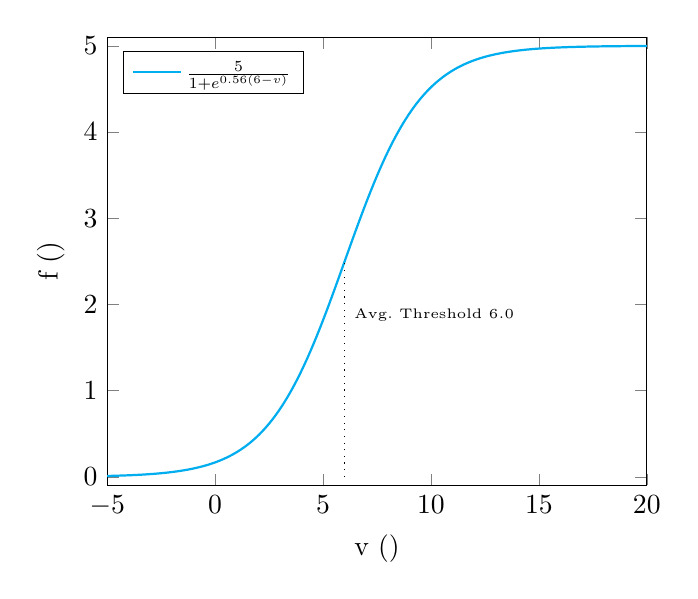
\begin{tikzpicture}
        \begin{axis}
            [
            xmin = -5, xmax = 20,
            ymin = -0.1, ymax = 5.1,
            xlabel = {v ($\SI{}{\milli\volt}$)},
            ylabel = {f ($\SI{}{\hertz}$)},
            legend pos=north west,
            legend style={nodes={scale=0.8, transform shape}},
            ],
            \addplot[
                domain = -5:20,
                samples = 200,
                smooth,
                thick,
                cyan,
            ] {5/(1+exp(0.56*(6-x)))};
            \legend{\( \frac{5}{1+e^{0.56(6-v)}} \)}
            \draw [dotted] ([xshift=0.0cm]axis cs:6,0) -- ([yshift=0.0cm]axis cs:6,2.5) node[near end,right,font=\tiny]{
                Avg.\ Threshold $\SI{6.0}{\milli\volt}$};
        \end{axis}
    \end{tikzpicture}~\caption{Sigmoid (Eq.~\ref{eq:SigmJansenRit}) \cite{jansen_neurophysiologically-based_1993}}
    \label{fig:Sigmoid}
\end{figure}

\subsubsection{PSP-Blocks}
In Physics, Linear Time-Invariant Systems (LTI systems) are oftentimes used to describe the response of
electrical circuits to arbitrary input signals.
They consist of a kernel function (or impulse-response function)
that models the system's response to a single unit-impulse.
The aforementioned PSP-Blocks are an LTI system fully represented by an impulse response function describing a PSP
relative to the onset of a pulse.
Since the PSP differs depending on the type of cell (excitatory or inhibitory),
there are two different impulse-response functions.
The parameters Jansen \& Rit used for the EPSP (Eq.~\ref{eq:ExcImpResJansenRit}) and IPSP (Eq.~\ref{eq:InhImpResJansenRit})
were based on results from van Rotterdam et al.~\cite{van_rotterdam_model_1982} and are given in Table~\ref{tab:psp_params}.
The respective plots are visualized in Fig.~\ref{fig:PSPPlot}.
%TODO: explain how the parameters can be tuned to achieve differnt results, and how that relatates to actual neurobiology
\begin{table}[H]
    \centering
    \begin{tabular}{ |c|c|c|c| }
        \hline
        \multicolumn{2}{|c|}{Parameter} & Default Value & Unit \\
        \hline
        \hline
        Exc. max. amplitude / $e$          & \(A\) & \(3.25\) & \(\SI{}{\milli\volt}\) \\
        \hline
        %TODO: EXPLAIN 'LUMPED'!!!!
        Lumped repr. of sum of exc. delays & \(a\) & \(100\)  & \(\SI{}{\hertz}\) \\
        \hline
        Inh. max. amplitude / $e$          & \(B\) & \(22\)   & \(\SI{}{\milli\volt}\) \\
        \hline
        Lumped repr. of sum of inh. delays & \(b\) & \(50\)   & \(\SI{}{\hertz}\) \\
        \hline
    \end{tabular}
    \caption{Parameters of the PSP Blocks}
    \label{tab:psp_params}
\end{table}

Excitatory impulse response:
\begin{equation}
    h_e(t) = \begin{cases}
                 Aate^{-at} & \mbox{ } t \geq 0 \\
                 0 & \mbox{ } t < 0
    \end{cases} \label{eq:ExcImpResJansenRit}
\end{equation}

Inhibitory impulse response:
\begin{equation}
    h_i(t) = \begin{cases}
                 Bbte^{-bt} & \mbox{ } t \geq 0 \\
                 0 & \mbox{ } t < 0
    \end{cases} \label{eq:InhImpResJansenRit}
\end{equation}



\begin{figure}[H]
    \centering
    \pgfplotsset{compat = newest}
    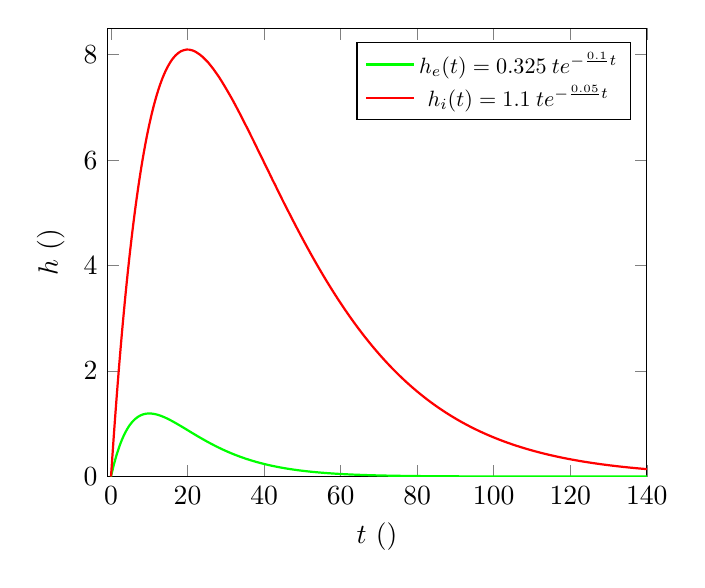
\begin{tikzpicture}
        \begin{axis}
            [
            xmin = -1, xmax = 140,
            ymin = 0, ymax = 8.5,
            xlabel = {$t$ ($\SI{}{\milli\second}$)},
            ylabel = {$h$ ($\SI{}{\milli\volt}$)},
            legend pos=north east,
            legend style={nodes={scale=0.8, transform shape}},
            ],
            \addplot[
                domain = 0:140,
                samples = 200,
                smooth,
                thick,
                green,
            ] {3.25*0.1*x*e^(-0.1*x)};
            \addplot[
                domain = 0:140,
                samples = 200,
                smooth,
                thick,
                red,
            ] {22*0.05*x*e^(-0.05*x)};

            \legend{
                $h_e(t)=0.325\frac{\SI{}{\milli\volt}}{\SI{}{\milli\second}} te^{-\frac{0.1}{\SI{}{\milli\second}}t} $,
                $ h_i(t)=1.1\frac{\SI{}{\milli\volt}}{\SI{}{\milli\second}} te^{-\frac{0.05}{\SI{}{\milli\second}}t} $
            };

        \end{axis}
    \end{tikzpicture}

    \caption{
        \textbf{Impulse Response Functions:}
        Note the small \textcolor{green}{EPSP}  (Eq.~\ref{eq:ExcImpResJansenRit}) and the
        large \textcolor{red}{IPSP}  (Eq.~\ref{eq:InhImpResJansenRit})~\parencite{jansen_neurophysiologically-based_1993}} \
    \label{fig:PSPPlot}
\end{figure}
Jansen and Rit~\cite{jansen_neurophysiologically-based_1993} justify the difference in amplitude by
referencing Lopes da Silva et al.~\cite{lopes_da_silva_models_1976} and stating that inhibitory neurons
synapse closer to the somata of pyramidal cells (often on the cell body) than excitatory cells,
increasing the effect of an inhibitory neuron about 10-fold.

The output of the Linear System defined by the PSP-Blocks is calculated by a convolution (denoted by $\ast$) of the
incoming impulse density $x(t)$ with the impulse response function $h(t)$.
For the excitatory PSP this means:\\
\begin{align}
    \overbrace{y(t)}^{\text{PSP}} = \overbrace{h_e(t)}^{\text{impulse response}} \ast \overbrace{x(t)}^{\text{impulse density}} \label{eq:convolution}
\end{align}
%%%%
% REMARK: CONVOLUTION
%%%%

\newremarkimg{Convolution}{
\begin{wrapfigure}[12]{r}{0.5\textwidth}
    \centering
    \includegraphics[width=0.45\textwidth]{Figures/convolution/wikipedia-convolution}
    \caption{\textbf{Convolution:} The area enclosed by $f(\tau)$ and $g(t-\tau)$ is the value of $(f\ast g)(t)$.\\
    \hrulefill \\
    \textit{By Cmglee - Own work, CC BY-SA 3.0  \url{https://commons.wikimedia.org/w/index.php?curid=20206883}}}
    \label{fig:Convolution}
\end{wrapfigure}
}
{
    The convolution of two functions $f(t)$ and $g(t)$ is defined as the integral of their product after one function
    has been reversed and shifted (Fig.~\ref{fig:Convolution}):
    \[f(t) \ast g(t)= \int_{-\infty}^{+\infty}f(\tau)g(t-\tau) d\tau\]
    If $f(t)$ is a unit-impulse $\delta(t)$ (in our case, this would mean that each cell of the previous population
    is firing a single action potential at the same time) the result is just $g(t)$ - a
    single full-amplitude PSP:
    \[\delta(t) \ast g(t)= \int_{-\infty}^{+\infty}\delta(\tau)g(t-\tau) d\tau = g(t)\]
    In the general case, this process can be used to mathematically model the integration of
    incoming action potential densities in the soma.\\[1em]
    Importantly, the Convolution Theorem states that the convolution of $f(t)$ and $g(t)$ becomes a
    simple multiplication when applying the Laplace Transform:
    \[\mathscr{L}\{f(t) \ast g(t)\}= \mathscr{L}\{f(t)\}\mathscr{L}\{g(t)\} = F(s)G(s)\]
    That means you can calculate a convolution with the inverse Laplace-Transform of the multiplication of
    the functions' individual Laplace-Transforms:
    \[f(t) \ast g(t)= \mathscr{L}^{-1}\{F(s)G(s)\}\]
%\end{remark}
}
Since the convolution in the time-domain is a computationally heavy operation,
it is oftentimes faster to transform the equation into the Laplace-Domain (see Eq.~\ref{eq:laplace_domain}),
apply the Convolution Theorem to perform the multiplication there,
and transform the results back to the time-domain.
This results in a second order differential equation (Eq.~\ref{eq:sec_ord_nmm}) that
can be efficiently solved by numerical integration.
To obtain this form, we need the Laplace transform $H_e(s)$ (in this context also called \textit{Transfer Function})
of our response function $h_e(t)$:
\[H_e(s) =\mathscr{L}\{h_e(t)\}  = \mathscr{L}\{Aate^{-at} \} = \frac{Aa}{(s+a)^2} = \frac{Aa}{s^2+2as+a^2}\label{eq:laplace_h_e}\]
With that, we can start to transform our initial equation (Eq.~\ref{eq:convolution}) into the desired Second Order System:
\begin{alignat}{5}
    &                                           & &&          \overbrace{y(t)}^{\text{PSP}} \quad &&=& \quad \overbrace{h_e(t)}^{\text{impulse response}} \ast \overbrace{x(t)}^{\text{impulse density}} \nonumber \\[1em]
    &                                           & \omit\rlap{applying the Laplace-Transform eliminates the convolution:}                 \nonumber \\[1em]
    &  \stackrel{\mathscr{L}}{\iff} \qquad      & &&                             Y(s) \quad &&=& \quad \overbrace{H_e(s)}^{\text{transfer function}} \cdot X(s)  \label{eq:laplace_domain} \\
    &  \iff                                     & &&                             Y(s) \quad &&=& \quad \frac{AaX(s)}{s^2+2as+a^2}  \nonumber \\
    &  \iff                                     & &&               (s^2+2as+a^2) Y(s) \quad &&=& \quad AaX(s) \nonumber \\
    &  \iff                                     & &&          s^{2}Y(s)+2asY(s)+a^{2}Y(s) \quad &&=& \quad AaX(s) \nonumber \\[1em]
    \omit\rlap{reversing the Laplace-Transform yields a differential equation in the time domain:}     \nonumber \\[1em]
    &  \stackrel{\mathscr{L}^{-1}}{\iff} \qquad & && \ddot{y}(t)+2a\dot{y}(t)+a^{2}y(t) \quad &&=& \quad Aax(t) \nonumber \\
    &  \iff                                     & &&                      \ddot{y}(t) \quad &&=& \quad Aax(t)-2a\dot{y}(t)-a^{2}y(t)  \label{eq:sec_ord_nmm} \\[1em]
    &                                           & \omit\rlap{which can be expressed as a system of two coupled first order equations:}                 \nonumber \\[1em]
    &                                           & &&                       \dot{y}(t) \quad &&=& \quad z(t)  \label{eq:y_t}\\
    &                                           & &&                       \dot{z}(t) \quad &&=& \quad Aax(t)-2az(t)-a^{2}y(t)   \label{eq:z_t}
\end{alignat}
where $y(t)$ is the resulting PSP and $x(t)$ the incoming pulse density.
This works analogously for the inhibitory case with $h_i(t)$.

\subsubsection{Full Linear System}

Taking the two first order equations for $\dot{y}(t)$ (Eq.~\ref{eq:y_t}) and $\dot{z}(t)$ (Eq.~\ref{eq:z_t})
and the Block diagram (Fig.~\ref{fig:JRBlockColored}) as a base,
we can now state the equations for the full Jansen-Rit Model with it's three populations.
Each PSP-Block $h(t)$ needs it's own system of coupled differential equations.
The value of $x(t)$ can be easily taken from the Block Diagram. $y_0(t)$ is the EPSP received by
both the EIN and IIN population, while $y_1(t)$ is the EPSP and $y_2(t)$ the IPSP received by the PC population:
\begin{equation}
    \begin{aligned}
        \dot{y}_0(t) &= z_0(t) \\
        \dot{z}_0(t) &= \fcolorbox{cyan!80}{cyan!5}{ $ Aa Sigm[y_1(t) - y_2(t)] - 2az_0(t) - a^{2}y_0(t) $}\\
        \dot{y}_1(t) &= z_1(t) \\
        \dot{z}_1(t) &= \fcolorbox{green!80}{green!5}{$ Aa(p(t) + C_{2}Sigm[C_{1}y_0(t)]) - 2az_1(t) - a^{2}y_1(t)$}\\
        \dot{y}_2(t) &= z_2(t) \\
        \dot{z}_2(t) &= \fcolorbox{red!80}{red!5}{$ Bb(C_{4}Sigm[C_{3}y_0(t)]) - 2bz_2(t) -b^{2}y_2(t)$} \\
    \end{aligned}\label{eq:jr_nmm_system}
\end{equation}

\begin{figure}[H]
    \centering
    \begin{tikzpicture}[
        pc/.style={draw=cyan!80, fill=cyan!5},
        ein/.style={draw=green!80, fill=green!5},
        iin/.style={draw=red!80, fill=red!5},
        pcLabel/.style={font=\small,text=cyan!80},
        einLabel/.style={font=\small,text=green!80},
        iinLabel/.style={font=\small,text=red!80},
        rectNode/.style={draw=black!80, thick},
        roundNode/.style={circle, draw=black!80, thick},
        ]
	    
 % Nodes
\node[rectNode, pc] (SigmPC) [label={[pcLabel]:PC}] {$Sigm$};
\node[rectNode, pc] (PSPPC) [right=1.8cm of SigmPC.east]{$h_e(t)$};
\node[rectNode, ein] (SigmEIN) [above=2cm of SigmPC.center, label={[einLabel]:EIN}]{$Sigm$};
\node[rectNode, iin] (SigmIIN) [below=2cm of SigmPC.center, label={[iinLabel]:IIN}]{$Sigm$};
\node[rectNode, ein] (PSPEIN) [above left= 0.5cm and 2cm of SigmPC.west]{$h_e(t)$};
\node[rectNode, iin] (PSPIIN) [below left= 0.5cm and 2cm of SigmPC.west]{$h_i(t)$};
\node[rectNode, rounded corners=3mm, ein] (ext) [left=2cm of PSPEIN.west, label={[einLabel]:Ext.}]{$p(t)$};
\node (inpIPSP) [left=0.8cm of PSPIIN.west]{};
\node (outPPSP) [right=1.2cm of PSPPC.east]{};
\node[roundNode, ein] (c1) [right=2cm of SigmEIN.east]{$C_1$};
\node[roundNode, ein] (c2) [left=2cm of SigmEIN.west]{$C_2$};
\node[roundNode, iin] (c3) [right=2cm of SigmIIN.east]{$C_3$};
\node[roundNode, iin] (c4) [left=2cm of SigmIIN.west]{$C_4$};

% add PC
\node[roundNode, pc] (addPC) [left=0.8cm of SigmPC.west]{};
\draw[-, black!80, thick, pc] (addPC.north west) -- (addPC.south east);
\draw[-, black!80, thick, pc] (addPC.north east) -- (addPC.south west);
% add Excitatory
\node[roundNode, ein] (addExc) [left=0.8cm of PSPEIN.west]{};
\draw[-, black!80, thick, ein] (addExc.north west) -- (addExc.south east);
\draw[-, black!80, thick, ein] (addExc.north east) -- (addExc.south west);

% add PC -> Sigm PC -> PSP PC
\draw[-{Stealth[scale=1.5]}, pc] (addPC.east) -- (SigmPC.west)node[coordinate, pos=0.3](measurepoint){};
\draw[-{Stealth[scale=1.5]}, pc] (SigmPC.east) -- (PSPPC.west);

% PSP PC -> y0
\draw[-{Stealth[scale=1.5]}, pc] (PSPPC.east) -- (outPPSP.center) node[pos=0.5, above, pcLabel]{\small$y_0(t)$};

% y0 -> C1 -> Sigm EIN
\draw[-{Stealth[scale=1.5]}, ein, fill=none] (outPPSP.center) |- (c1.east);
\draw[-{Stealth[scale=1.5]}, ein] (c1.west) -- (SigmEIN.east);

% y0 -> C3 -> Sigm IIN
\draw[-{Stealth[scale=1.5]}, iin, fill=none] (outPPSP.center) |- (c3.east);
\draw[-{Stealth[scale=1.5]}, iin] (c3.west) -- (SigmIIN.east);


% Sigm EIN -> c2 -> add EXC
\draw[-{Stealth[scale=1.5]}, ein] (SigmEIN.west) -- (c2.east);
\draw[-{Stealth[scale=1.5]}, ein, fill=none] (c2.west) -| (addExc.north) node[pos=0.9, right]{\small$+$};
% external -> add EXC
\draw[-{Stealth[scale=1.5]}, ein] (ext.east) -- (addExc.west) node[pos=0.9, above]{\small$+$};

% add EXC -> PSP EIN
\draw[-{Stealth[scale=1.5]}, ein] (addExc.east) -- (PSPEIN.west);
% PSP EIN -> add PC
\draw[-{Stealth[scale=1.5]}, ein, fill=none] (PSPEIN.east) -| (addPC.north) node[pos=1, left]{\small$+$} node[pos=0.4, above, einLabel]{\small$y_1(t)$};

% Sigm IIN -> C4 -> PSP IIN
\draw[-{Stealth[scale=1.5]}, iin] (SigmIIN.west) -- (c4.east);
\draw[-, iin, fill=none] (c4.west) -| (inpIPSP.center);
\draw[-{Stealth[scale=1.5]}, iin] (inpIPSP.center) -- (PSPIIN.west);
% PSP IIN -> add PC
\draw[-{Stealth[scale=1.5]}, iin, fill=none] (PSPIIN.east) -| (addPC.south) node[pos=1, left]{\small$-$} node[pos=0.4, below, iinLabel]{\small$y_2(t)$};

% electrode
\draw (measurepoint.north) -- (-1.1,1)node[coordinate,pos=0.9](a){} -- (-0.8,0.9)node[coordinate, pos=0.5](b){} -- cycle;
\node (signal)[above right=0.2cm and 2.1cm of a]{\tiny recorded Signal};
\draw (b.center) |- (signal.west);



\end{tikzpicture}
    \caption{Colored Block diagram, visualizing the components of (Eq.~\ref{eq:jr_nmm_system})}
    \label{fig:JRBlockColored}
\end{figure}

\subsubsection{Model Input}

The model input $p(t)$ represents the average activity of populations outside the modeled
column that synapse on the columns PC population.
Since this activity's source is so diverse, it is modeled by white noise ($120-\SI{320}{\hertz}$).

%\begin{wrapfigure}[5]{r}{0.32\textwidth}
\begin{figure}[H]
    \centering
    \pgfplotsset{compat = newest}
    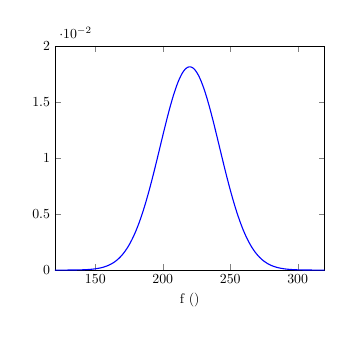
\begin{tikzpicture}[scale=0.5]
        \begin{axis}
            [
            xmin = 120, xmax = 320,
            ymin = 0, ymax = 0.02,
            xlabel = {f ($\SI{}{\hertz}$)},
            legend pos=outer north east,
            legend style={nodes={scale=1.2, transform shape}},
            ],
            \addplot[
                domain = 120:320,
                samples = 200,
                smooth,
                thick,
                blue,
            ]{(exp(-0.5*((x-220)/22)^2))/(22*sqrt(2*pi))};
            %\legend{$\frac{1}{22\sqrt{2\pi}}e^{-\frac{1}{2}(\frac{x-220}{22})^2}$};

        \end{axis}
    \end{tikzpicture}

    \caption{
        \textbf{Input distribution.}
        The input frequency representing $p(t)$ is sampled from a normal distribution with $\mu=220$ and $\sigma=22$}
    \label{fig:ModelInput}
        %\end{wrapfigure}
\end{figure}

\subsubsection{Connectivity Constants}\label{subsubsec:connectivity_constants}

A sensible choice for the Connectivity Constants $C_1$ to $C_4$ was determined by Jansen and Rit empirically by
defining a histologically motivated relationship between them ($C = C_1 = \frac{C_2}{0.8} = \frac{C_3}{0.25} =
\frac{C_4}{0.25}$) and varying $C$ until the system produced the desired natural alpha-like activity at $C=C_1=135
\Rightarrow C_2=108; C_3=C_4=33.75$.
Varying $C$ can account for common synaptic phenomena like
neurotransmitter depletion~\parencite{jansen_electroencephalogram_1995}.


\subsubsection{Model Output}
Simulated data from $y_1-y_2$ while varying $C$ is plotted in Fig.~\ref{fig:jr_c_sweep},
which is perfectly reproducing ~\cite[Fig. 3]{jansen_electroencephalogram_1995}.
The desired alpha-activity is clearly visible for $C = 135$,
which led Jansen \& Rit to their choice of default parameters mentioned in Sec.~\ref{subsubsec:connectivity_constants}.
The other plots give an insight into the models capabilities of producing varying forms of activity,
but in this work we will not further explore variations of $C$.
An interesting phenomenon is, however,
that very low and very high connectivity both leads to the system being entirely noise-driven,
which produces signals with identical form, but different amplitude for different values of $C$ (compare $C=1350$ and $C=68$),
as long as they are supplied with identical input.
All signals in Fig.~\ref{fig:jr_c_sweep} were generated with the same pre-sampled random input.

Fig.~\ref{fig:jr_psd} shows the Power Spectral Density (PSD) of the chosen signal and the corresponding spectrogram for a
60 second simulation session is given in Fig.~\ref{fig:jr_spec}.
It is clearly visible that the signal is mainly composed of a single sinusoidal component at  $\approx \SI{11}{\hertz}$.
\begin{figure}[H]
    \centering
    \subfloat[\textbf{JR Model Output for varying $C$.} \\
    Well defined alpha-activity is visible at $C=135$.\\
    ]{\label{fig:jr_c_sweep}
        \resizebox{!}{10cm}{
            \begin{tikzpicture}
                \pgfplotsset{
                %% Axis
                    scale only axis,
                    width=0.8\linewidth,
                    height=2cm,
                    every axis/.append style={
                        line width=1pt,
                        tick style={line width=0.8pt},
                        %   grid style={dashed, black!20},
                        %  grid=major,
                    },
        %               %% X-Axis
                    xmin=1.0,
                    xmax=3,
                }
                \begin{groupplot}
                    [
                    group style={
                        group size=1 by 6,
                        vertical sep=2mm,
                        xlabels at=edge bottom,
                        xticklabels at=edge bottom,
                    },
                    yticklabel style={
                        /pgf/number format/fixed,
                        /pgf/number format/precision=2
                    },
                    legend style={nodes={scale=0.8, transform shape}, thin},
                    legend image post style={scale=0},
                    xlabel=$t (\SI{}{\second})$
                    ]
        %           \pgfplotsinvokeforeach{0,1,2,3,4,5}{
        %             \nextgroupplot
        %             \addplot [line width=1pt,solid,color=cyan] table[x=x,y= c#1 ,col sep=comma]{data/test135.csv};
        %          }
                    \nextgroupplot
                    \addplot [line width=1pt,solid] table[x=x,y=c0 ,col sep=comma]{data/simple_c_sweep.csv};
                    \legend{$C=68$};
                    \nextgroupplot
                    \addplot [line width=1pt,solid] table[x=x,y=c1 ,col sep=comma]{data/simple_c_sweep.csv};
                    \legend{$C=128$};
                    \nextgroupplot
                    \addplot [line width=1pt,solid] table[x=x,y=c2 ,col sep=comma]{data/simple_c_sweep.csv};
                    \legend{$C=135$};
                    \nextgroupplot[ylabel=v ($\SI{}{\micro\volt}$), every axis y label/.append style={at=(ticklabel cs:1.0)}]
                    \addplot [line width=1pt,solid] table[x=x,y=c3 ,col sep=comma]{data/simple_c_sweep.csv};
                    \legend{$C=270$};
                    \nextgroupplot
                    \addplot [line width=1pt,solid] table[x=x,y=c4 ,col sep=comma]{data/simple_c_sweep.csv};
                    \legend{$C=675$};
                    \nextgroupplot
                    \addplot [line width=1pt,solid] table[x=x,y=c5 ,col sep=comma]{data/simple_c_sweep.csv};
                    \legend{$C=1350$};

                \end{groupplot}
            \end{tikzpicture}
        }
    }
    \hfill
    \subfloat[\textbf{PSD of JR Model Output.} \\
                     ($C=135$, Multitapered)]{\label{fig:jr_psd}
        \resizebox{7cm}{5.3cm}{
            \pgfplotsset{compat = newest}
            \begin{tikzpicture}[scale=0.5]
                \begin{axis}
                    [
                    ],
                    \addplot [line width=.5pt,solid, cyan]
                        table[x=x,y=y ,col sep=comma]{data/methodology/psd_multitaper_jr.csv};

                \end{axis}
            \end{tikzpicture}

        }
    }
    \subfloat[\textbf{Spectrogram of JR Model Output.} \\
                     ($C=135$)]{\label{fig:jr_spec}
        \resizebox{7.5cm}{!}{
            \import{data/rest_sim}{JR_REST_60.pgf}
        }
    }
    %\hfill
    \caption{\textbf{Properties of JR Model Output}}
    \label{fig:jr_model_out_props}
\end{figure}

\pagebreak

\subsection{The Sub-Population-Extension by David and Friston}\label{subsec:the-david-and-friston-model}
While the JR model succeeds in generating realistic alpha activity,
real EEG Signals contain much richer spectra~\parencite{steriade_impact_2001}.
David and Friston~\cite{david_neural_2003} proposed a modification to the JR model,
that could produce a more realistic frequency spectrum by adding sub-populations to the model.
They can be tuned individually to produce oscillations in different frequencies.

\subsubsection{Introducing sub-populations}

David and Friston slightly redefine the impulse response function $h(t)$ (Eq.~\ref{eq:ExcImpResJansenRit})
in the PSP-Blocks by introducing the parameters $H$ and $\tau$ (see Table~\ref{tab:davidfriston}),
which are just a minor alteration of $A$ and $a$.
\[ h(t)=Aate^{-at} => h(t)=\frac{H}{\tau}te^{-\frac{1}{\tau}} \]
Before tweaking these parameters to produce slower or faster kinetics,
they define the products $H_e\tau_e=\SI{0.0325}{\milli\volt\second}$ and $H_i\tau_i=\SI{0.44}{\milli\volt\second}$ as constants.
This is done to preserve the oscillatory behavior of each population~\parencite{david_neural_2003}.
When varying $\tau$, $H$ is therefore adjusted
accordingly ($H_e=\frac{\SI{0.0325}{\milli\volt\second}}{\tau_e}$, $H_i=\frac{\SI{0.44}{\milli\volt\second}}{\tau_i}$).
\begin{table}[H]
    \centering
    \begin{tabular}{ |c|c|c|c|c| }
        \hline
        \multicolumn{2}{|c|}{Parameter} & Value & Unit & Relation to \parencite{jansen_electroencephalogram_1995} \\
        \hline
        \hline
        \rule{0pt}{3ex}Excitatory delays        & \(\tau_e\) & \(10\) & $\SI{}{\milli\second}$  & $ \tau_e = \frac{1}{a} $ \\[1.2ex]
        \hline
        \rule{0pt}{3ex}Inhibitory delays        & \(\tau_i\) & \(20\) & $\SI{}{\milli\second}$  & $ \tau_i = \frac{1}{b} $\\[1.2ex]
        \hline
        \rule{0pt}{3ex}Excitatory synaptic gain & \(H_e\)    & \(3.25\) & $\SI{}{\milli\volt}$ & $ H_e = A $ \\[1.2ex]
        \hline
        \rule{0pt}{3ex}Inhibitory synaptic gain & \(H_i\)    & \(22\)   & $\SI{}{\milli\volt}$ & $ H_i = B $ \\[1.2ex]
        \hline
    \end{tabular}
    \caption{Parameters of the PSP Blocks after David \& Friston~\cite{david_neural_2003}}
    \label{tab:davidfriston}
\end{table}
\fcolorbox{red}{red!10}{\parbox{\textwidth}{
    \textbf{Attention:} For the remainder of this work, the indices $[0,\dots,N]$ for $y$, $h$, $\tau$ and $H$ refer only to
    the subpopulations within a single population.
    The indices used above in the formulation for the Simple Jansen-Rit Model (and the Block Diagram) should not
    be confused with these.
    However, $e$ and $i$ as indices still denote excitatory and inhibitory populations respectively.}} \\[1em]

\noindent
To introduce subpopulations, they split up the general impulse response function $h(t)$ in $N$ individual
sub-functions:
\[h_n(t) = \frac{H_n}{\tau_n}te^{-\frac{1}{\tau_n}}\]\\
\noindent
The previously defined general PSP-Block Equation:
\[y(t)=h(t)\ast x(t)\]
then becomes:
\[y(t)=\sum_{n=0}^{N}{(w_n \cdot h_n(t) \ast x(t))} \hspace{2em}
\text{with}
\hspace{2em} \sum_{n=0}^{N}w_n = 1 \hspace{2em}
\text{and}
\hspace{2em} 0 \leq w_n \leq 1\]
with N individually weighted ($w_n$) and parameterized ($h_n(t)$) subpopulations. \\
We can then declare:
\[y_n(t) = h_n(t) \ast x(t) \quad \text{and} \quad y(t) = \sum_{n=0}^{N} (w_{n}y_n)\]
which produces the following differential equations for a single PSP Block:

\begin{equation}
    \begin{aligned}
        \dot{y}_0(t) &= z_0(t) \\
        \dot{z}_0(t) &= \frac{H_0}{\tau_0} x(t) - \frac{2}{\tau_0}z_0(t) - \left(\frac{1}{\tau_0}\right)^{2}y_0(t)\\
        &\dots\\
        \dot{y}_N(t) &= z_N(t) \\
        \dot{z}_N(t) &= \frac{H_N}{\tau_N} x(t) - \frac{2}{\tau_N}z_N(t) - \left(\frac{1}{\tau_N}\right)^{2}y_N(t)\\
        y(t)         &= w_{0}y_0 + \dots + w_{N}y_N\\
    \end{aligned}\label{eq:davidfriston_subpops}
\end{equation}

\begin{figure}[H]
    \begin{tikzpicture}
	\node(sout){};
	\node[shape=rectangle, draw=black, left=0.3cm of sout.center] (SigmPC) {$x(t)$};
	
	\node[shape=rectangle, draw=black, above right=1cm and 2.5cm of sout.center] (H1) {$h_{e_0}(t)$};
	\node[shape=rectangle, draw=black, fill=white, below right=0.2cm and 0.2cm of H1.west] (H2) {$h_{e_1}(t)$};
	\node[shape=rectangle, draw=black, fill=white, below right=2cm and 0.8cm of H2.west] (HN) {$h_{e_N}(t)$};
	\draw[black!80, dots, dot diameter=4pt, dot spacing=25pt, shorten <=8pt, shorten >=8pt] (H2.south) -- (HN.north);
	\node[shape=rectangle, dotted, draw=black, fill=white, fill opacity=0.7, text opacity=1, below right=0.8cm and 0.4cm of H2.west] (Hen) {$h_{e_n}(t)$};
	
	
	\node[left=0.3cm of H1.west](x1){};
	\node[left=0.45cm of H2.west](x2){};
	\node[left=0.85cm of Hen.west](xen){};
	\node[left=1.3cm of HN.west](xN){};
	
	\node[shape=circle, draw=black, right=2cm of H1] (w1) {\small$w_0$};
	\node[shape=circle, draw=black,fill=white, right=2cm of H2] (w2) {\small$w_1$};
	\node[shape=circle, dotted, draw=black, right=2cm of Hen] (wen) {\small$w_n$};
	\node[shape=circle, draw=black, right=2cm of HN] (wN) {\small$w_N$};
	
	
	\node[right=1.1cm of w1.east](y1){};
	\node[right=0.9cm of w2.east](y2){};
	\node[right=0.5cm of wen.east](yen){};
	\node[right=0.001cm of wN.east](yN){};
	
	\node[shape=rectangle, draw=black, right=9cm of sout.center] (pout){$y(t)$};
	
	
	\draw[-] (SigmPC.east) -- (sout.center);
	
	\draw[-] (sout.center) .. controls +(3:1.2) and +(10:-1.5) .. (x1.center);
	\draw[-] (sout.center) .. controls +(3:1.2) and +(10:-1.5) .. (x2.center);
	\draw[-, dotted] (sout.center) .. controls +(3:1.2) and +(10:-1.5) .. (xen.center);
	\draw[-] (sout.center) .. controls +(3:1.2) and +(10:-1.5) .. (xN.center);
	
	
	\draw[->] (x1.center) |- (H1.west);
	\draw[->] (x2.center) |- (H2.west);
	\draw[->, dotted] (xen.center) |- (Hen.west);
	\draw[->] (xN.center) |- (HN.west);
	
	\draw[->] (H1.east) -- (w1.west) node [above, midway]{\tiny$y_0(t)$};
	\draw[->] (H2.east) -- (w2.west)node [above, midway]{\tiny$y_1(t)$};
	\draw[->, dotted] (Hen.east) -- (wen.west)node [above, midway]{\tiny$y_n(t)$};
	\draw[->] (HN.east) -- (wN.west)node [above, midway]{\tiny$y_N(t)$};
	
	
	
	\draw[-] (w1.east) |- (y1.center);
	\draw[-] (w2.east) |- (y2.center);
	\draw[-, dotted] (wen.east) |- (yen.center);
	\draw[-] (wN.east) |- (yN.center);
	
	\draw[->, very thin] (y1.center) .. controls +(3:1.2) and +(10:-1.5) .. (pout.west);
	\draw[->, very thin] (y2.center) .. controls +(3:1.2) and +(10:-1.5) .. (pout.west);
	\draw[->, dotted, thin] (yen.center) .. controls +(3:1.2) and +(10:-1.5) .. (pout.west);
	\draw[->, very thin] (yN.center) .. controls +(3:1.2) and +(10:-1.5) .. (pout.west);
	
\end{tikzpicture}
    \caption{Example of subpopulations ($h_{e_0}(t), \dots, h_{e_N}(t)$) forming an excitatory population $h_e(t)$}
    \label{fig:exc_subpops}
\end{figure}

\vspace{1em}
\noindent
David and Friston further propose an example with two subpopulations for each population.
The parameters are listed in Fig.~\ref{fig:PSPPlotDavidFriston}.
While the kinetics for the first subpopulation ($\tau_{e_0}, \tau_{i_0}$) in each population are still close
to those of the original populations ($\tau_e=10ms, \tau_i=20ms$, which produce alpha activity),
each of the second subpopulation's  ($\tau_{e_1}, \tau_{i_1}$) parameters were chosen to produce gamma activity.
The associated weights are  $w_0=0.8$ and $w_1=0.2$ for both populations,
favouring the original slower kinetics,
as this combination results in the most realistic frequency distribution according to the authors (compare Fig.~\ref{fig:df_psd}).

\begin{figure}[H]
    \centering
    \pgfplotsset{compat = newest}
    \begin{tikzpicture}
        \begin{axis}
            [
            xmin = 0, xmax = 140,
            ymin = 0, ymax = 55.1,
            xlabel = {$t$ ($\SI{}{\milli\second}$)},
            ylabel = {$h$ ($\SI{}{\milli\volt}$)},
            legend pos=north east,
            legend style={nodes={scale=0.8, transform shape}},
            domain = 0:140,
            samples = 200,
            smooth,
            thick,
            ],
            \addplot[green] {(3.01/10.8)*x*e^(-(1/10.8)*x)};\label{plot:line1}
            \addplot[blue] {(7.07/4.6)*x*e^(-(1/4.6)*x)};\label{plot:line2}
            \addplot[red] {(20/22)*x*e^(-(1/22)*x)};\label{plot:line3}
            \addplot[orange] {(151.72/2.9)*x*e^(-(1/2.9)*x)};\label{plot:line4}
            \coordinate (legend) at (axis description cs:0.97,0.97);
        \end{axis}
        \tiny
        \matrix [
            draw,
            matrix of nodes,
            anchor=north east,
        ] at (legend) {

            & $\tau$ &    $H$  \\
            \ref{plot:line1}$h_{e_0}(t)$ & 10.8ms &   3.0mV \\
            \ref{plot:line2}$h_{e_1}(t)$ &  4.6ms &   7.0mV \\
            \ref{plot:line3}$h_{i_0}(t)$ & 22.0ms &  20.0mV \\
            \ref{plot:line4}$h_{i_1}(t)$ &  2.9ms & 151.7mV \\
        };
    \end{tikzpicture}

    \caption{\textbf{PSP functions for subpopulations as proposed by David \& Friston~\cite{david_neural_2003}:} \\
        The subpopulations $h_{e_1}$ and $h_{i_1}$ are faster
        than the original populations and their slower variations in $h_{e_0}$ and $h_{i_0}$ and
        elicit activity with higher frequencies.
    }
    \label{fig:PSPPlotDavidFriston}
\end{figure}

\subsubsection{Model Output}
The values chosen by David \& Friston indeed produce a frequency distribution more
typical for EEG recordings \citationneeded,
with a broad distribution over the alpha and beta bands (Fig.~\ref{fig:df_psd}).
On average, the frequencies peak in alpha ($~\SI{12}{\hertz}$), as visible in the PSD plot,
however, the spectrogram (Fig.~\ref{fig:df_spec}) reveals fluctuations of the peak frequency
between the alpha and beta band over time.
The average frequency amplitude is harshly reduced compared to the JR model,
which becomes clear when scaling the JR model's PSD (Fig.~\ref{fig:jr_psd_rescaled})
and spectrogram (Fig.~\ref{fig:jr_spec_rescaled}) to the same value ranges.

\begin{figure}[H]
    \centering
    \subfloat[\textbf{PSD of DF Model Output.} (Multitapered)]{\label{fig:df_psd}
        \resizebox{7cm}{5.3cm}{
            \pgfplotsset{compat = newest}
            \begin{tikzpicture}[scale=0.5]
                \begin{axis}
                    [ymax=0.000000003
                    ],
                    \addplot [line width=.5pt,solid, cyan]
                        table[x=x,y=y ,col sep=comma]{data/methodology/psd_multitaper_df_35.csv};

                \end{axis}
            \end{tikzpicture}
        }
    }
    \subfloat[\textbf{Spectrogram of DF Model Output.}]{\label{fig:df_spec}
        \resizebox{7.5cm}{!}{
            \import{data/rest_sim}{DF_REST_60.pgf}
        }
    }
    \hfill
    \subfloat[\textbf{PSD of JR Model Output.} \\
              (see Fig.~\ref{fig:jr_psd})\\
              Scaled to match intensity for comparison]{\label{fig:jr_psd_rescaled}
        \resizebox{7cm}{5.3cm}{
            \pgfplotsset{compat = newest}
            \begin{tikzpicture}[scale=0.5]
                \begin{axis}
                    [ymax=0.000000003
                    ],
                    \addplot [line width=.5pt,solid, cyan]
                        table[x=x,y=y ,col sep=comma]{data/methodology/psd_multitaper_jr.csv};

                \end{axis}
            \end{tikzpicture}
        }
    }
    \subfloat[\textbf{Spectrogram of JR Model Output.}\\
              (see Fig.~\ref{fig:jr_spec})\\
              Scaled to match intensity for comparison]{\label{fig:jr_spec_rescaled}
        \resizebox{7.5cm}{!}{
            \import{data/rest_sim}{JR_REST_60_dfscale.pgf}
        }
    }
    \caption{\textbf{Properties of DF Model Output in comparison to JR model}}
    \label{fig:df_model_out_props}
\end{figure}